% Options for packages loaded elsewhere
\PassOptionsToPackage{unicode}{hyperref}
\PassOptionsToPackage{hyphens}{url}
%
\documentclass[
]{article}
\usepackage{amsmath,amssymb}
\usepackage{lmodern}
\usepackage{iftex}
\ifPDFTeX
  \usepackage[T1]{fontenc}
  \usepackage[utf8]{inputenc}
  \usepackage{textcomp} % provide euro and other symbols
\else % if luatex or xetex
  \usepackage{unicode-math}
  \defaultfontfeatures{Scale=MatchLowercase}
  \defaultfontfeatures[\rmfamily]{Ligatures=TeX,Scale=1}
\fi
% Use upquote if available, for straight quotes in verbatim environments
\IfFileExists{upquote.sty}{\usepackage{upquote}}{}
\IfFileExists{microtype.sty}{% use microtype if available
  \usepackage[]{microtype}
  \UseMicrotypeSet[protrusion]{basicmath} % disable protrusion for tt fonts
}{}
\makeatletter
\@ifundefined{KOMAClassName}{% if non-KOMA class
  \IfFileExists{parskip.sty}{%
    \usepackage{parskip}
  }{% else
    \setlength{\parindent}{0pt}
    \setlength{\parskip}{6pt plus 2pt minus 1pt}}
}{% if KOMA class
  \KOMAoptions{parskip=half}}
\makeatother
\usepackage{xcolor}
\IfFileExists{xurl.sty}{\usepackage{xurl}}{} % add URL line breaks if available
\IfFileExists{bookmark.sty}{\usepackage{bookmark}}{\usepackage{hyperref}}
\hypersetup{
  pdftitle={MATH 3F03 HW 1},
  pdfauthor={Matthew Bain (001406931)},
  hidelinks,
  pdfcreator={LaTeX via pandoc}}
\urlstyle{same} % disable monospaced font for URLs
\usepackage[margin=1in]{geometry}
\usepackage{color}
\usepackage{fancyvrb}
\newcommand{\VerbBar}{|}
\newcommand{\VERB}{\Verb[commandchars=\\\{\}]}
\DefineVerbatimEnvironment{Highlighting}{Verbatim}{commandchars=\\\{\}}
% Add ',fontsize=\small' for more characters per line
\usepackage{framed}
\definecolor{shadecolor}{RGB}{248,248,248}
\newenvironment{Shaded}{\begin{snugshade}}{\end{snugshade}}
\newcommand{\AlertTok}[1]{\textcolor[rgb]{0.94,0.16,0.16}{#1}}
\newcommand{\AnnotationTok}[1]{\textcolor[rgb]{0.56,0.35,0.01}{\textbf{\textit{#1}}}}
\newcommand{\AttributeTok}[1]{\textcolor[rgb]{0.77,0.63,0.00}{#1}}
\newcommand{\BaseNTok}[1]{\textcolor[rgb]{0.00,0.00,0.81}{#1}}
\newcommand{\BuiltInTok}[1]{#1}
\newcommand{\CharTok}[1]{\textcolor[rgb]{0.31,0.60,0.02}{#1}}
\newcommand{\CommentTok}[1]{\textcolor[rgb]{0.56,0.35,0.01}{\textit{#1}}}
\newcommand{\CommentVarTok}[1]{\textcolor[rgb]{0.56,0.35,0.01}{\textbf{\textit{#1}}}}
\newcommand{\ConstantTok}[1]{\textcolor[rgb]{0.00,0.00,0.00}{#1}}
\newcommand{\ControlFlowTok}[1]{\textcolor[rgb]{0.13,0.29,0.53}{\textbf{#1}}}
\newcommand{\DataTypeTok}[1]{\textcolor[rgb]{0.13,0.29,0.53}{#1}}
\newcommand{\DecValTok}[1]{\textcolor[rgb]{0.00,0.00,0.81}{#1}}
\newcommand{\DocumentationTok}[1]{\textcolor[rgb]{0.56,0.35,0.01}{\textbf{\textit{#1}}}}
\newcommand{\ErrorTok}[1]{\textcolor[rgb]{0.64,0.00,0.00}{\textbf{#1}}}
\newcommand{\ExtensionTok}[1]{#1}
\newcommand{\FloatTok}[1]{\textcolor[rgb]{0.00,0.00,0.81}{#1}}
\newcommand{\FunctionTok}[1]{\textcolor[rgb]{0.00,0.00,0.00}{#1}}
\newcommand{\ImportTok}[1]{#1}
\newcommand{\InformationTok}[1]{\textcolor[rgb]{0.56,0.35,0.01}{\textbf{\textit{#1}}}}
\newcommand{\KeywordTok}[1]{\textcolor[rgb]{0.13,0.29,0.53}{\textbf{#1}}}
\newcommand{\NormalTok}[1]{#1}
\newcommand{\OperatorTok}[1]{\textcolor[rgb]{0.81,0.36,0.00}{\textbf{#1}}}
\newcommand{\OtherTok}[1]{\textcolor[rgb]{0.56,0.35,0.01}{#1}}
\newcommand{\PreprocessorTok}[1]{\textcolor[rgb]{0.56,0.35,0.01}{\textit{#1}}}
\newcommand{\RegionMarkerTok}[1]{#1}
\newcommand{\SpecialCharTok}[1]{\textcolor[rgb]{0.00,0.00,0.00}{#1}}
\newcommand{\SpecialStringTok}[1]{\textcolor[rgb]{0.31,0.60,0.02}{#1}}
\newcommand{\StringTok}[1]{\textcolor[rgb]{0.31,0.60,0.02}{#1}}
\newcommand{\VariableTok}[1]{\textcolor[rgb]{0.00,0.00,0.00}{#1}}
\newcommand{\VerbatimStringTok}[1]{\textcolor[rgb]{0.31,0.60,0.02}{#1}}
\newcommand{\WarningTok}[1]{\textcolor[rgb]{0.56,0.35,0.01}{\textbf{\textit{#1}}}}
\usepackage{longtable,booktabs,array}
\usepackage{calc} % for calculating minipage widths
% Correct order of tables after \paragraph or \subparagraph
\usepackage{etoolbox}
\makeatletter
\patchcmd\longtable{\par}{\if@noskipsec\mbox{}\fi\par}{}{}
\makeatother
% Allow footnotes in longtable head/foot
\IfFileExists{footnotehyper.sty}{\usepackage{footnotehyper}}{\usepackage{footnote}}
\makesavenoteenv{longtable}
\usepackage{graphicx}
\makeatletter
\def\maxwidth{\ifdim\Gin@nat@width>\linewidth\linewidth\else\Gin@nat@width\fi}
\def\maxheight{\ifdim\Gin@nat@height>\textheight\textheight\else\Gin@nat@height\fi}
\makeatother
% Scale images if necessary, so that they will not overflow the page
% margins by default, and it is still possible to overwrite the defaults
% using explicit options in \includegraphics[width, height, ...]{}
\setkeys{Gin}{width=\maxwidth,height=\maxheight,keepaspectratio}
% Set default figure placement to htbp
\makeatletter
\def\fps@figure{htbp}
\makeatother
\usepackage[normalem]{ulem}
% Avoid problems with \sout in headers with hyperref
\pdfstringdefDisableCommands{\renewcommand{\sout}{}}
\setlength{\emergencystretch}{3em} % prevent overfull lines
\providecommand{\tightlist}{%
  \setlength{\itemsep}{0pt}\setlength{\parskip}{0pt}}
\setcounter{secnumdepth}{-\maxdimen} % remove section numbering
\newlength{\cslhangindent}
\setlength{\cslhangindent}{1.5em}
\newlength{\csllabelwidth}
\setlength{\csllabelwidth}{3em}
\newlength{\cslentryspacingunit} % times entry-spacing
\setlength{\cslentryspacingunit}{\parskip}
\newenvironment{CSLReferences}[2] % #1 hanging-ident, #2 entry spacing
 {% don't indent paragraphs
  \setlength{\parindent}{0pt}
  % turn on hanging indent if param 1 is 1
  \ifodd #1
  \let\oldpar\par
  \def\par{\hangindent=\cslhangindent\oldpar}
  \fi
  % set entry spacing
  \setlength{\parskip}{#2\cslentryspacingunit}
 }%
 {}
\usepackage{calc}
\newcommand{\CSLBlock}[1]{#1\hfill\break}
\newcommand{\CSLLeftMargin}[1]{\parbox[t]{\csllabelwidth}{#1}}
\newcommand{\CSLRightInline}[1]{\parbox[t]{\linewidth - \csllabelwidth}{#1}\break}
\newcommand{\CSLIndent}[1]{\hspace{\cslhangindent}#1}
\ifLuaTeX
  \usepackage{selnolig}  % disable illegal ligatures
\fi

\title{MATH 3F03 HW 1}
\author{Matthew Bain (001406931)}
\date{19/09/22}

\begin{document}
\maketitle

{
\setcounter{tocdepth}{2}
\tableofcontents
}
\begin{verbatim}
## $knitr
## $knitr$opts_knit
## $knitr$opts_knit$bookdown.internal.label
## [1] TRUE
## 
## $knitr$opts_knit$kable.force.latex
## [1] TRUE
## 
## 
## $knitr$opts_chunk
## $knitr$opts_chunk$dev
## [1] "png"
## 
## $knitr$opts_chunk$dpi
## [1] 96
## 
## $knitr$opts_chunk$fig.width
## [1] 7
## 
## $knitr$opts_chunk$fig.height
## [1] 5
## 
## $knitr$opts_chunk$fig.retina
## [1] 2
## 
## 
## $knitr$knit_hooks
## NULL
## 
## $knitr$opts_hooks
## NULL
## 
## $knitr$opts_template
## NULL
## 
## 
## $pandoc
## $pandoc$to
## [1] "html"
## 
## $pandoc$from
## [1] "markdown+autolink_bare_uris+tex_math_single_backslash"
## 
## $pandoc$args
##  [1] "--wrap"                                                                                              
##  [2] "preserve"                                                                                            
##  [3] "--standalone"                                                                                        
##  [4] "--section-divs"                                                                                      
##  [5] "--table-of-contents"                                                                                 
##  [6] "--toc-depth"                                                                                         
##  [7] "3"                                                                                                   
##  [8] "--template"                                                                                          
##  [9] "/Library/Frameworks/R.framework/Versions/4.1-arm64/Resources/library/bookdown/templates/gitbook.html"
## [10] "--highlight-style"                                                                                   
## [11] "pygments"                                                                                            
## [12] "--number-sections"                                                                                   
## 
## $pandoc$keep_tex
## [1] FALSE
## 
## $pandoc$latex_engine
## [1] "pdflatex"
## 
## $pandoc$ext
## NULL
## 
## $pandoc$lua_filters
## [1] "/Library/Frameworks/R.framework/Versions/4.1-arm64/Resources/library/bookdown/rmarkdown/lua/custom-environment.lua"
## [2] "/Library/Frameworks/R.framework/Versions/4.1-arm64/Resources/library/rmarkdown/rmarkdown/lua/pagebreak.lua"        
## [3] "/Library/Frameworks/R.framework/Versions/4.1-arm64/Resources/library/rmarkdown/rmarkdown/lua/latex-div.lua"        
## [4] "/Library/Frameworks/R.framework/Versions/4.1-arm64/Resources/library/rmarkdown/rmarkdown/lua/anchor-sections.lua"  
## 
## 
## $keep_md
## [1] FALSE
## 
## $clean_supporting
## [1] FALSE
## 
## $df_print
## [1] "default"
## 
## $pre_knit
## function (...) 
## {
##     op(base(...), overlay(...))
## }
## <bytecode: 0x13bd71488>
## <environment: 0x11e7c1f98>
## 
## $post_knit
## function (...) 
## {
##     op(base(...), overlay(...))
## }
## <bytecode: 0x13bd71488>
## <environment: 0x11e7c1748>
## 
## $pre_processor
## function (...) 
## {
##     op(base(...), overlay(...))
## }
## <bytecode: 0x13bd71488>
## <environment: 0x11e7c0fd8>
## 
## $intermediates_generator
## function (original_input, intermediates_dir) 
## {
##     copy_render_intermediates(original_input, intermediates_dir, 
##         !self_contained)
## }
## <bytecode: 0x13bd1c798>
## <environment: 0x12a4cd0b8>
## 
## $post_processor
## function (metadata, input, output, clean, verbose) 
## {
##     if (is.function(post)) 
##         output = post(metadata, input, output, clean, verbose)
##     on.exit(write_search_data(), add = TRUE)
##     x = read_utf8(output)
##     x = x[x != "div.sourceCode { margin: 1em 0; }"]
##     write_utf8(x, output)
##     move_files_html(output, lib_dir)
##     output2 = split_chapters(output, gitbook_page, global_numbering, 
##         split_by, split_bib, gb_config, split_by)
##     if (file.exists(output) && !same_path(output, output2)) 
##         file.remove(output)
##     move_files_html(output2, lib_dir)
##     output2
## }
## <bytecode: 0x10e6749b8>
## <environment: 0x12a425c08>
## 
## $on_exit
## function () 
## options(opts)
## <bytecode: 0x119176208>
## <environment: 0x11e7c9678>
## 
## $bookdown_output_format
## [1] "html"
## 
## attr(,"class")
## [1] "rmarkdown_output_format"
\end{verbatim}

\begin{verbatim}
## undoing setup
\end{verbatim}

\begin{verbatim}
## function (content, global = FALSE) 
## {
##     content = resolve_ref_links_html(content)
##     res = parse_fig_labels(content, global)
##     content = res$content
##     ref_table = c(res$ref_table, parse_section_labels(content))
##     m = gregexpr("(?<!\\\\)@ref\\(([-:[:alnum:]]+)\\)", content, 
##         perl = TRUE)
##     refs = regmatches(content, m)
##     for (i in seq_along(refs)) {
##         if (length(refs[[i]]) == 0) 
##             next
##         ref = ref_to_number(refs[[i]], ref_table, FALSE)
##         if (is_img_line(content[i])) 
##             ref = strip_html(ref)
##         refs[[i]] = ref
##     }
##     regmatches(content, m) = refs
##     content
## }
## <bytecode: 0x11be257e8>
## <environment: namespace:bookdown>
\end{verbatim}

\newpage

\hypertarget{some-snippets-to-useincorporate}{%
\section{some snippets to
use/incorporate}\label{some-snippets-to-useincorporate}}

\hypertarget{some-snippets}{%
\subsection{some snippets}\label{some-snippets}}

\[ 
\begin{align} 
  g(X_{n}) & = g(\theta) + g'({\tilde{\theta}})(X_{n} - \theta) (\#eq:res0) \\
  \sqrt{n}[g(X_{n}) - g(\theta)] 
  & = g'\left({\tilde{\theta}}\right) \sqrt{n}[X_{n} -\theta ] (\#eq:res1) \\
  & = g'\left({\tilde{\theta}}\right) \sqrt{n}[X_{n} -\theta ] (\#eq:res2)
\end{align} 
\]

\[
\begin{align}   g(X_{n}) & = g(\theta) + g'({\tilde{\theta}})(X_{n} - \theta) \notag \\  \sqrt{n}[g(X_{n}) - g(\theta)] &  = g'\left({\tilde{\theta}}\right) \sqrt{n}[X_{n} -\theta ] (\#eq:hello)\end{align}
\]

\leavevmode\vadjust pre{\hypertarget{pyth}{}}%
For a right triangle, if \(c\) denotes the length of the hypotenuse and
\(a\) and \(b\) denote the lengths of the other two sides, we have

\[a^2 + b^2 = c^2\]

For a right triangle, if \(c\) denotes the length of the hypotenuse and
\(a\) and \(b\) denote the lengths of the other two sides, we have

\[a^2 + b^2 = c^2\]

\leavevmode\vadjust pre{\hypertarget{CZ}{}}%
\[
\forall ~ x \in z ~\exists ~ y~  s.t. ~ ...
\]

\[
\begin{align}   g(X_{n}) & = g(\theta) + g'({\tilde{\theta}})(X_{n} - \theta) \notag \\  \sqrt{n}[g(X_{n}) - g(\theta)] &  = g'\left({\tilde{\theta}}\right) \sqrt{n}[X_{n} -\theta ] (\#eq:pythagor)\end{align}
\]

\href{https://groups.google.com/g/knitr/c/OMvT03PtGPM}{This forum
post}\footnote{forum post:
  \url{https://groups.google.com/g/knitr/c/OMvT03PtGPM}} contains some
very useful insights on configuring RMD settings using HTML to
auto-number equations by default. More details on the
\href{https://docs.mathjax.org/en/latest/web/typeset.html\#tex-reset}{MathJax
documentation}\footnote{\href{https://docs.mathjax.org/en/latest/web/typeset.html\#tex-reset}{MathJax
  doc:
  {[}https://docs.mathjax.org/en/latest/web/typeset.html\textbackslash\#tex-reset{]}(https://docs.mathjax.org/en/latest/web/typeset.html\#tex-reset)\{.uri\}}}
page.

\begin{figure}
\centering
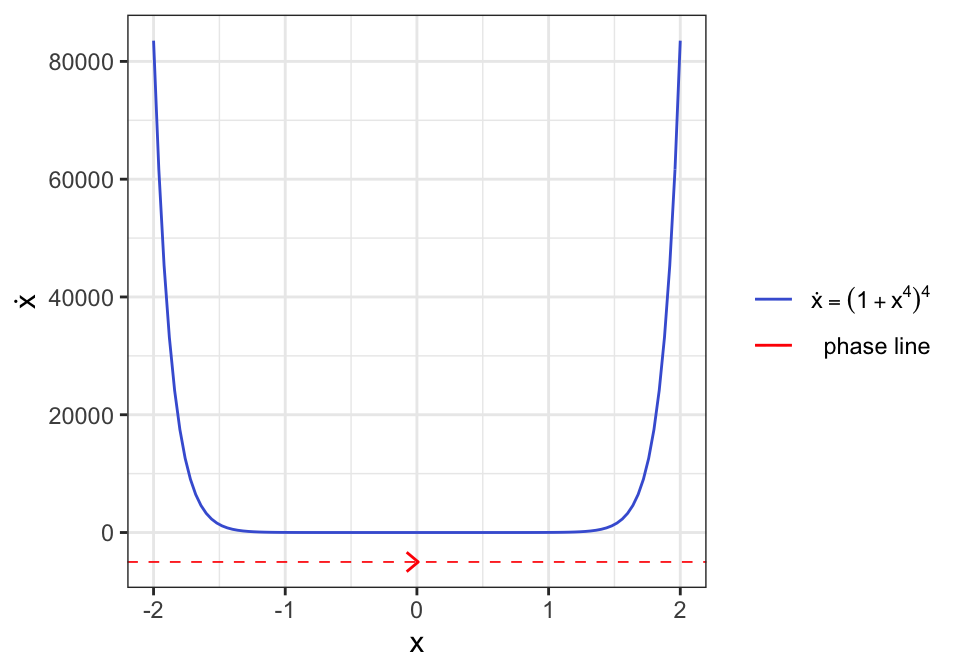
\includegraphics{figures/q1-f1-1.png}
\caption{Question (A): plot of \(\dot{x}\)}
\end{figure}

See figure @ref(fig:q1-f1) (this is a figure cross-reference).

See equation @ref(eq:res2)

\hypertarget{snippets-section-2}{%
\section{snippets section 2}\label{snippets-section-2}}

\hypertarget{some-snippets-2}{%
\subsection{some snippets 2}\label{some-snippets-2}}

For a right triangle, if \(c\) denotes the length of the hypotenuse and
\(a\) and \(b\) denote the lengths of the other two sides, we have

\[a^2 + b^2 = c^2\]

\hypertarget{snippets-section-3}{%
\section{snippets section 3}\label{snippets-section-3}}

\hypertarget{some-snippets-3}{%
\subsection{some snippets 3}\label{some-snippets-3}}

\emph{\textbf{Assumptions}:}

\begin{itemize}
\tightlist
\item
  \(\gamma: (\alpha,\beta) \rightarrow \mathbb{R}^n, \bar{\gamma}: (\alpha',\beta') \rightarrow \mathbb{R}^n\)
\end{itemize}

\textbf{\emph{Background}}:

\begin{itemize}
\item
  we write \(\gamma \sim \bar{\gamma}\) if and only if \(\bar{\gamma}\)
  is a \textbf{reparametrization} of \(\gamma\)

  \begin{itemize}
  \tightlist
  \item
    i.e., if \(\exists\) a \textbf{diffeomorphism}
    \(\phi: (\alpha',\beta') \rightarrow (\alpha,\beta) ~ \text{such that} ~ \gamma \circ \phi = \bar{\gamma}\)
  \end{itemize}
\end{itemize}

\hypertarget{question-1a}{%
\subsection{Question 1a}\label{question-1a}}

\emph{\textbf{Prove}: that} \(\sim\) \emph{defines an
\textbf{equivalence relation} on the set of all parametrized curves in}
\(\mathbb{R}^n\)\emph{.}

\begin{description}
\item[\emph{proof.}]
\emph{Recall.} In order for \(\sim\) to be an \textbf{equivalence
relation} it must satisfy three properties:

\begin{enumerate}
\def\labelenumi{\arabic{enumi}.}
\tightlist
\item
  reflexivity: \(\gamma \sim \gamma\)
\item
  symmetry: \(\gamma \sim \bar{\gamma} \iff \bar{\gamma} \sim \gamma\)
\item
  transitivity:
  \(\gamma \sim \bar{\gamma} ~ \text{and} ~ \bar{\gamma} \sim \bar{\bar{\gamma}} \implies \gamma \sim \bar{\bar{\gamma}}\)
\end{enumerate}

Thus, to complete this proof we will check each of these properties in
turn.

\textbf{1) Reflexive}

To show that \(\gamma\) is a reparametrization of itself, we have to
find a reparametrization map \(\phi\) such that
\(\gamma(\phi(t)) = \bar{\gamma}(t) ~~ \text{for all} ~~ t \in (\alpha,\beta)\).

Since in this case \(\gamma = \bar{\gamma}\), let \(\phi\) be the
identity map, \(\phi: t \in (\alpha,\beta) \rightarrow (\alpha,\beta)\)
defined by \(\phi(t) = t\), with inverse \(\phi^{-1}(t) = \phi(t)\) such
that \(\phi^{-1} \circ \phi(t) = t\).

Then,

\[
\gamma(\phi(t)) = \gamma(t) \text{,}
\]

and \(\phi^{-1}(t) = \phi(t)\) is smooth, since \(\phi(t)\) is
continuously differentiable, with

\[
\frac{d\phi}{dt} = \dot{\phi} = 1 ~~ \text{and} ~~ \frac{d^k\phi}{dt^k} = 0 ~~ \text{for all} ~~ k > 1 \text{.}
\]

Thus, \(\sim\) is reflexive.

\textbf{2) Symmetric}

\emph{Notice}: Given \(\gamma \sim \bar{\gamma}\), i.e.,
\(\gamma(\phi(t)) = \bar{\gamma}(t)\), there exists a \(\phi'(t)\) such
that \(\bar{\gamma}(\phi'(t)) = \gamma(t)\) for all
\(t \in (\alpha,\beta)\).

Namely, \(\phi'(t) = \phi^{-1}(t)\) (which exists since \(\phi\) is a
diffeomorphism): \(\bar{\gamma}(\phi^{-1}(t)) = \gamma(t)\).

Thus, \(\sim\) is symmetric.

\textbf{3) Transitive}

Let \(\phi(t), \phi'(t)\) be reparametrization maps satisfying the
following \(\text{for all} ~~ t \in (\alpha,\beta)\):

\[
\gamma \circ \phi = \gamma(\phi(t)) = \gamma(\bar{t}) = \bar{\gamma}(t), \\
\bar{\gamma} \circ \phi' = \bar{\gamma}(\phi'(t)) = \bar{\gamma}(\bar{t}) = \bar{\bar{\gamma}}(t).
\]

Then, to show that \(\sim\) is transitive, we must show that there
exists exists a \(\phi''(t)\) such that

\[
\gamma \circ \phi'' = \gamma(\phi''(t)) = \gamma(\bar{\bar{t}}) =  \bar{\bar{\gamma}}(t) \text{.}
\]

\emph{Notice:} We find \(\phi''\) by composing the reparametrization
maps \(\phi'\) and \(\phi\):

Let \(\phi'(\phi(t)) = \phi'(\bar{t}) = \phi''(t) = \bar{\bar{t}}\).
Then,

\[
\gamma \circ \phi'' = \gamma(\phi''(t)) = \gamma(\phi'(\bar{t})) = \gamma(\bar{\bar{t}}) = \bar{\bar{\gamma}}(t) \text{.}
\]

By the chain rule, since \(\phi, \phi'\) are smooth maps with smooth
inverses, \(\phi'' = \phi' \circ \phi\) is also smooth, with a smooth
inverse defined by \((\phi'')^{-1} = (\phi'(\phi(t)))^{-1}\).

Thus, \(\sim\) is transitive.

Therefore, \(\sim\) is an equivalence relation

\[
\tag*{$\square$}
\]
\end{description}

\hypertarget{main-doc}{%
\section{main doc}\label{main-doc}}

\hypertarget{principles}{%
\subsection{principles}\label{principles}}

\hypertarget{general}{%
\subsubsection{general}\label{general}}

\begin{itemize}
\tightlist
\item
  all dependencies imported at the top of the document with brief
  comment on their utility
\item
  YAML uses distill format (default overall web/article/blog layout \&
  format/style - TOC, references, annotations, LaTeX + MathJax
  integration, figure/code presentation, syntax highlighting, etc.) and
  references bibtex file containing all references (books, manuals,
  articles) and LaTeX header file loading in any required packages for
  generating the desired math equations
\item
  use 2 header levels (sections and subsections) and place all body text
  under the subsection level - use bolded text for any `header' below
  this level
\item
  bold/italicize key terms/phrases
\item
  all images, tables, figures come with identifiers (for within-doc
  referencing) and informative but concise (usually no more than 1-2
  lines) captions
\item
  all critical equations contain numerical index for easy referencing
  within document
\item
  parenthetical comments appear as marginal notes (`asides', in the
  language of distill), along with minor images/figures - less pressing
  comments appear as annotations
\item
  link to all referenced web/wiki articles (non-scientific)
\item
  follow standard APA referencing and reference official documentation
  for all libraries used
\item
  all references, annotations are listed at the foot of document and can
  be previewed by hovering the mouse over their corresponding in-text
  citations/numbers
\end{itemize}

\hypertarget{document-setup}{%
\subsection{document setup}\label{document-setup}}

\hypertarget{default-knitr-options}{%
\subsubsection{default knitr options}\label{default-knitr-options}}

\begin{Shaded}
\begin{Highlighting}[]
\NormalTok{knitr}\SpecialCharTok{::}\NormalTok{opts\_chunk}\SpecialCharTok{$}\FunctionTok{set}\NormalTok{(}\AttributeTok{echo =} \ConstantTok{TRUE}\NormalTok{)}
\end{Highlighting}
\end{Shaded}

\hypertarget{critical-libraries}{%
\subsubsection{critical libraries}\label{critical-libraries}}

\begin{Shaded}
\begin{Highlighting}[]
\FunctionTok{library}\NormalTok{(viridis) }\CommentTok{\# generates awesome colour maps, ex:}
\FunctionTok{library}\NormalTok{(highr) }\CommentTok{\# applies syntax highlighting to ? *** }
\FunctionTok{library}\NormalTok{(ggplot2)}
\FunctionTok{library}\NormalTok{(formatR) }\CommentTok{\# expands R formatting options}

\NormalTok{clrs }\OtherTok{=} \FunctionTok{viridis}\NormalTok{(}\DecValTok{10}\NormalTok{)}

\NormalTok{knitr}\SpecialCharTok{::}\NormalTok{opts\_chunk}\SpecialCharTok{$}\FunctionTok{set}\NormalTok{(}\AttributeTok{tidy.opts =} \FunctionTok{list}\NormalTok{(}\AttributeTok{width.cutoff =} \DecValTok{60}\NormalTok{), }\AttributeTok{tidy =} \ConstantTok{TRUE}\NormalTok{) }\CommentTok{\# enable code wrapping in code output within knitted documents? ***}
\end{Highlighting}
\end{Shaded}

\hypertarget{key-ideas}{%
\subsection{key ideas}\label{key-ideas}}

\hypertarget{definition-theorem-remark.}{%
\subsubsection{definition, theorem,
remark.}\label{definition-theorem-remark.}}

\begin{description}
\item[\emph{definition.} \textbf{Equivalence relation.}]
An \textbf{equivalence relation} is a \(\forall ~ x \in z ~ \exists\)
\item[\emph{theorem.} \textbf{Fermat's last theorem.}]
x
\item[\emph{remark.} \textbf{Properties of symmetric matrices.}]
x
\end{description}

\hypertarget{proof}{%
\subsubsection{proof}\label{proof}}

\begin{description}
\item[\emph{proof.}]
\textbf{part 1}

\emph{Recall.} If we \ldots{}

\[
\begin{align}
    3+x &=4 && \text{(solve for} \space x \text{)} (\#eq:help)\\
    x &=4-3 && \text{(subtract 3 from both sides)}\\
    x &=1   && \text{(yielding the solution.)}
\end{align}
\]

We begin by

\[
\int_{10}^{\infty}\int_{0}^{2x + 3} 2z(4x + \sin(2z + 4)) ~ dx
\]

\emph{notice}. If we make \ldots{}

This completes the proof \(\tag*{\)\square\$\}\$
\end{description}

\hypertarget{math3-4}{%
\subsection[math ]{\texorpdfstring{math\footnote{some nice examples of
  LaTeX equation presentation styles in RMD:
  \url{https://www.math.mcgill.ca/yyang/regression/RMarkdown/example.html}}
\footnote{showcases a wide variety of useful mathematical objects
  displayed in LaTeX (derivatives, limits, statistical notation,
  integrals, sequences, etc.):
  \url{https://rpruim.github.io/s341/S19/from-class/MathinRmd.html}}}{math }}\label{math3-4}}

\hypertarget{aligned-equations-comments-indices}{%
\subsubsection{(aligned) equations, comments,
indices}\label{aligned-equations-comments-indices}}

\emph{(some examples. critical mathematical objects: vectors \&
matrices; functions \& parametric eq'ns \& vector fields; integrals \&
derivatives) (T: still to add: integrals \& derivatives; figure out
document-wide auto-numbering - 1,2,3,\ldots{} - of equations (and
suppressing on particular lines))}

\[
\begin{align}
  3 + x & = 4 && \text{(solve for} ~ x \text{)} (\#eq:res5) \\
  x & = 4 - 3 && \text{(subtract 3 from both sides)} \\
  x & = 1   && \text{(yielding the solution)}
\end{align}
\]

\[
\begin{equation}   
  f\left(k\right) = \binom{n}{k} p^k(1 - p)^{n-k}
\end{equation}
\]

\[
\left[\begin{matrix}
  a & b \\
  c & d \\
\end{matrix}\right]
\left[\begin{matrix}
  {cx} \\ 
  y 
\end{matrix}\right] = 
\left[\begin{matrix}
  {c} \cos \left(t \right) \\ 
  \sin \left(t \right) 
\end{matrix}\right], ~ t = 0…1
\]

\[
\begin{equation}
  r = \frac{1}{n-1} \sum_{i=1}^{n} \frac{(X_i - \bar {X})(Y_i - \bar{Y})}{S_xS_y} 
\tag{by commutativity} \\    
\end{equation}
\]

\hypertarget{define-latex-macros}{%
\subsubsection{define LaTeX macros}\label{define-latex-macros}}

\begin{Shaded}
\begin{Highlighting}[]
\CommentTok{\%\% define some macros (\textbackslash{}Xbar, \textbackslash{}sumn)}
\FunctionTok{\textbackslash{}def\textbackslash{}Xbar}\NormalTok{\{}\FunctionTok{\textbackslash{}overline}\NormalTok{\{X\}\_}\FunctionTok{\textbackslash{}bullet}\NormalTok{\}}
\FunctionTok{\textbackslash{}def\textbackslash{}sumn}\NormalTok{\{}\FunctionTok{\textbackslash{}sum}\NormalTok{\_\{i=1\}\^{}\{n\}\}}
\end{Highlighting}
\end{Shaded}

\[
\begin{align}
\sum_{i=1}^{n}\left(X_i - \overline{X}_\bullet\right)
  & = \sum_{i=1}^{n}X_i - \sum_{i=1}^{n}\overline{X}_\bullet && \text{(comment 1)} \\
  & = \sum_{i=1}^{n}X_i - n \overline{X}_\bullet && \text{(comment 2)} (\#eq:yep) \\
  & = \sum_{i=1}^{n}X_i - \sum_{i=1}^{n}X_i (\#eq:yepyep)\\
  & = 0
\end{align} 
\]

\textbf{\emph{Some style notes}}

\begin{itemize}
\item
  add spaces: \texttt{\textasciitilde{}}
\item
  indentation within environments: begin each new line with two spaces
\item
  define macros:
  \texttt{\textbackslash{}def{[}\textbackslash{}define\ object{]}\{\ {[}modifiers{]}\ \}}
\item
  new line: \texttt{\textbackslash{}\textbackslash{}}
\item
  aligned equation environment:
  \texttt{\textbackslash{}begin\{align\}\ {[}body{]}\ \textbackslash{}end(align\}}
\item
  add aligned comments/equations: precede aligned text with \texttt{\&},
  math w/ \texttt{\&\&}
\item
  number equation (right align numerical index):
  \texttt{\textbackslash{}tag\{\ {[}index{]}\ \}}

  \begin{itemize}
  \tightlist
  \item
    remove parentheses: insert \texttt{*} after
    \texttt{\textbackslash{}tag}
  \end{itemize}
\item
  insert math within text/tag `sub-environment' (delimited by
  `\texttt{\{\}}': insert `\texttt{\$\ \$}' around
  `\texttt{\textbackslash{}}' commands
\item
  don't include blank lines within LaTeX environments (this leads to
  errors)
\item
  close out macros (\texttt{\textbackslash{}...}) with
  \texttt{\textbackslash{};} - more generally use to close out compact
  term \& add space before next
\item
  create bracketed term:
  \texttt{\$\textbackslash{}left(\ {[}term{]}\ \textbackslash{}right)\$}
\item
  assign label to equation \texttt{(\textbackslash{}\#eq:label)} (within
  equation environment)
\end{itemize}

\hypertarget{asides}{%
\subsubsection{asides}\label{asides}}

This content will appear in the gutter of the article.

\hypertarget{lists}{%
\subsubsection{lists}\label{lists}}

(\emph{N: use tight formatting}) \{style=``color: \#A3EAFF''\}

\textbf{numbered}

\begin{enumerate}
\def\labelenumi{\arabic{enumi}.}
\item
  number 1
\item
  number 2
\item
  number 3

  \begin{enumerate}
  \def\labelenumii{\alph{enumii})}
  \tightlist
  \item
    part a
  \item
    part b
  \item
    part c
  \end{enumerate}
\end{enumerate}

\textbf{bulleted}

\begin{itemize}
\tightlist
\item
  bullet 1
\item
  bullet 2
\item
  bullet 3
\end{itemize}

\textbf{checklist}

\begin{itemize}
\item[$\square$]
  item 1

  \begin{itemize}
  \tightlist
  \item[$\boxtimes$]
    item 1a
  \end{itemize}
\item[$\square$]
  item 2
\end{itemize}

\hypertarget{citations-in-textparenthetical}{%
\subsubsection{citations
(in-text/parenthetical)}\label{citations-in-textparenthetical}}

R Core Team (2020) found this. (Azzalini and Bowman 1990),
\href{https://bookdown.org/yihui/rmarkdown-cookbook/html-css.html}{link}.

\hypertarget{footnote}{%
\subsubsection{footnote}\label{footnote}}

this is a footnote\footnote{link:
  \url{https://en.wikipedia.org/wiki/Main_Page}}

\hypertarget{text-formatting}{%
\subsubsection{text formatting}\label{text-formatting}}

This is \sout{strikethrough}, subscript\textsubscript{1},
superscript\textsuperscript{2}, \textsc{small caps,} \texttt{code}

\hypertarget{coloured-underlined-text}{%
\subsubsection{coloured, underlined
text}\label{coloured-underlined-text}}

Roses are \textbackslash textcolor\{red\}\{red\}, violets are
\textbackslash textcolor\{blue\}\{blue\}.

\hypertarget{quotes}{%
\subsubsection{quotes}\label{quotes}}

\begin{quote}
If you never lie you never need to remember a thing.

- Mark Twain, 1857
\end{quote}

\hypertarget{cross-reference-key-ideaequationvisualsection}{%
\subsubsection{cross-reference (key
idea/equation/visual/section)}\label{cross-reference-key-ideaequationvisualsection}}

\protect\hyperlink{river}{image reference}

@ref()

\hypertarget{visuals}{%
\subsection{visuals}\label{visuals}}

\hypertarget{images}{%
\subsubsection{images}\label{images}}

\emph{(properly referenced w/ annotation - Google Arts \& Culture CC +
artist/title/year)}

\begin{figure}
\hypertarget{river}{%
\centering
\includegraphics[width=4.6875in,height=\textheight]{images/Childe Hassam - The Concord Meadow.jpg}
\caption{a lovely river}\label{river}
}
\end{figure}

\hypertarget{visual-asides}{%
\subsubsection{visual asides}\label{visual-asides}}

\begin{Shaded}
\begin{Highlighting}[]
\FunctionTok{library}\NormalTok{(ggplot2)}
\FunctionTok{ggplot}\NormalTok{(mtcars, }\FunctionTok{aes}\NormalTok{(hp, mpg)) }\SpecialCharTok{+} \FunctionTok{geom\_point}\NormalTok{() }\SpecialCharTok{+} \FunctionTok{geom\_smooth}\NormalTok{()}
\end{Highlighting}
\end{Shaded}

\begin{figure}
\centering
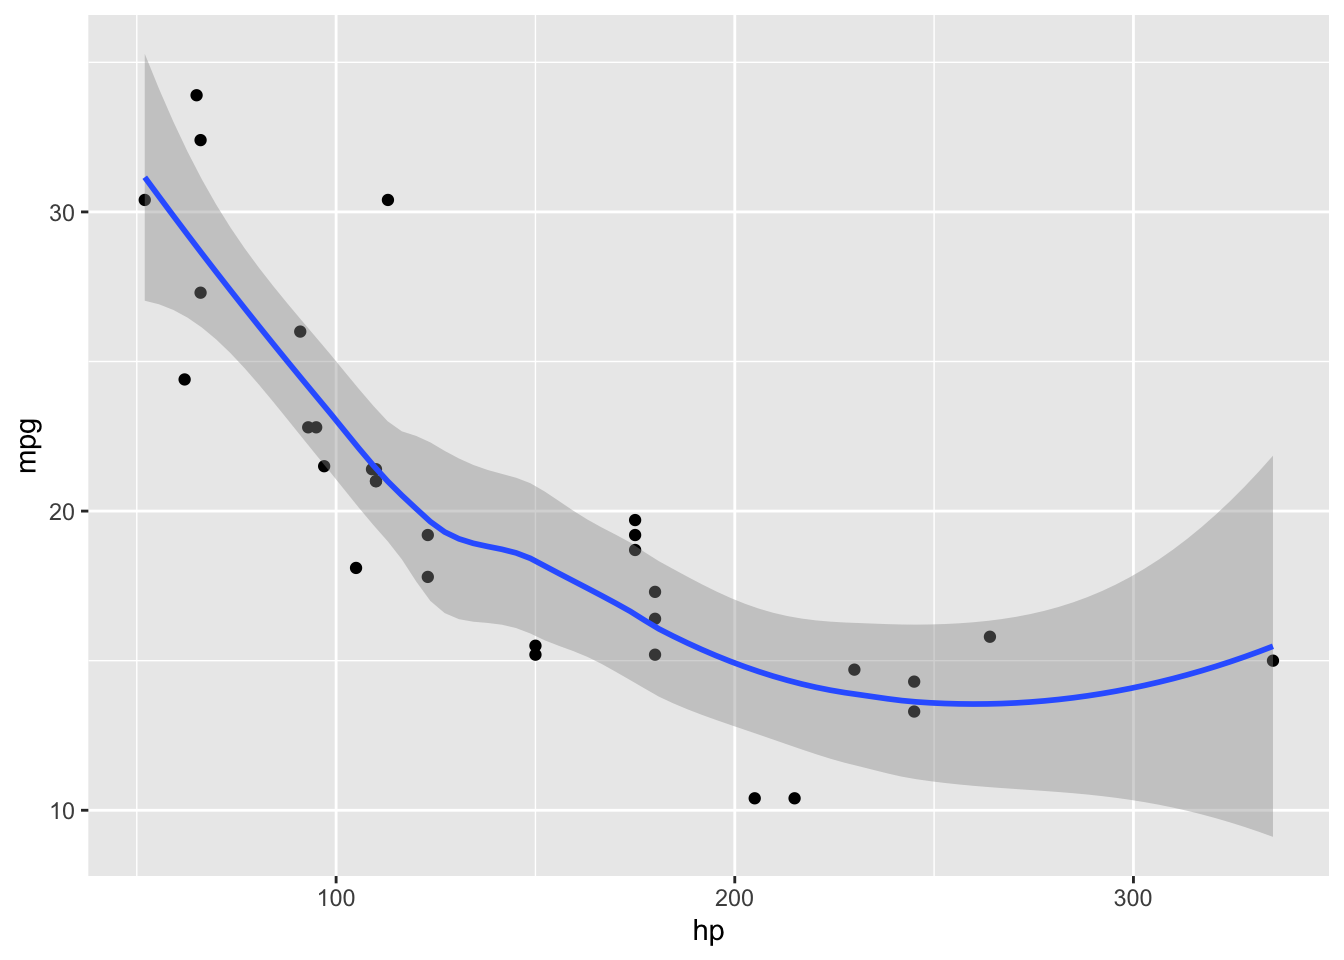
\includegraphics{figures/unnamed-chunk-5-1.png}
\caption{Figure}
\end{figure}

\hypertarget{tables}{%
\subsection{tables}\label{tables}}

\hypertarget{manually-generated}{%
\subsubsection{manually generated}\label{manually-generated}}

\emph{(adding col/rows, populating locally)}

\begin{longtable}[]{@{}lll@{}}
\caption{this is a table.}\tabularnewline
\toprule
Col1 & Col2 & Col3 \\
\midrule
\endfirsthead
\toprule
Col1 & Col2 & Col3 \\
\midrule
\endhead
x = 2 & this is what we do here & hello \\
& & y \\
& & x \\
\bottomrule
\end{longtable}

\hypertarget{imported-sortsearchable}{%
\subsubsection{imported \&
sort/searchable}\label{imported-sortsearchable}}

\hypertarget{figures}{%
\subsection{figures}\label{figures}}

\hypertarget{ggplot-plots}{%
\subsubsection{\texorpdfstring{\texttt{ggplot}
plots}{ggplot plots}}\label{ggplot-plots}}

\begin{figure}
\centering
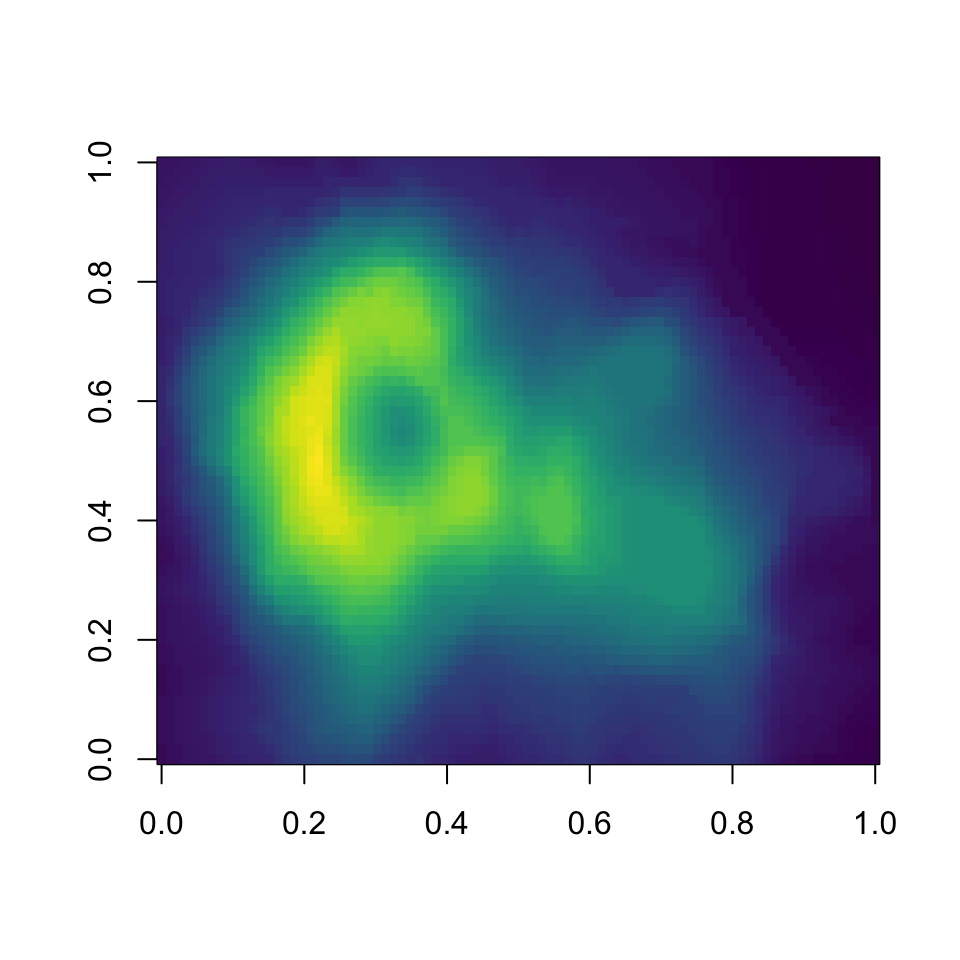
\includegraphics{figures/my-chunk-1.png}
\caption{color palette from the viridis package. Plot displays a contour
map of the Maunga Whau volcano.}
\end{figure}

\begin{Shaded}
\begin{Highlighting}[]
\FunctionTok{image}\NormalTok{(volcano, }\AttributeTok{col =} \FunctionTok{viridis}\NormalTok{(}\DecValTok{200}\NormalTok{, }\AttributeTok{option =} \StringTok{"A"}\NormalTok{))  }\CommentTok{\# using \textasciigrave{}magma\textasciigrave{} pallette}
\end{Highlighting}
\end{Shaded}

\begin{figure}
\centering
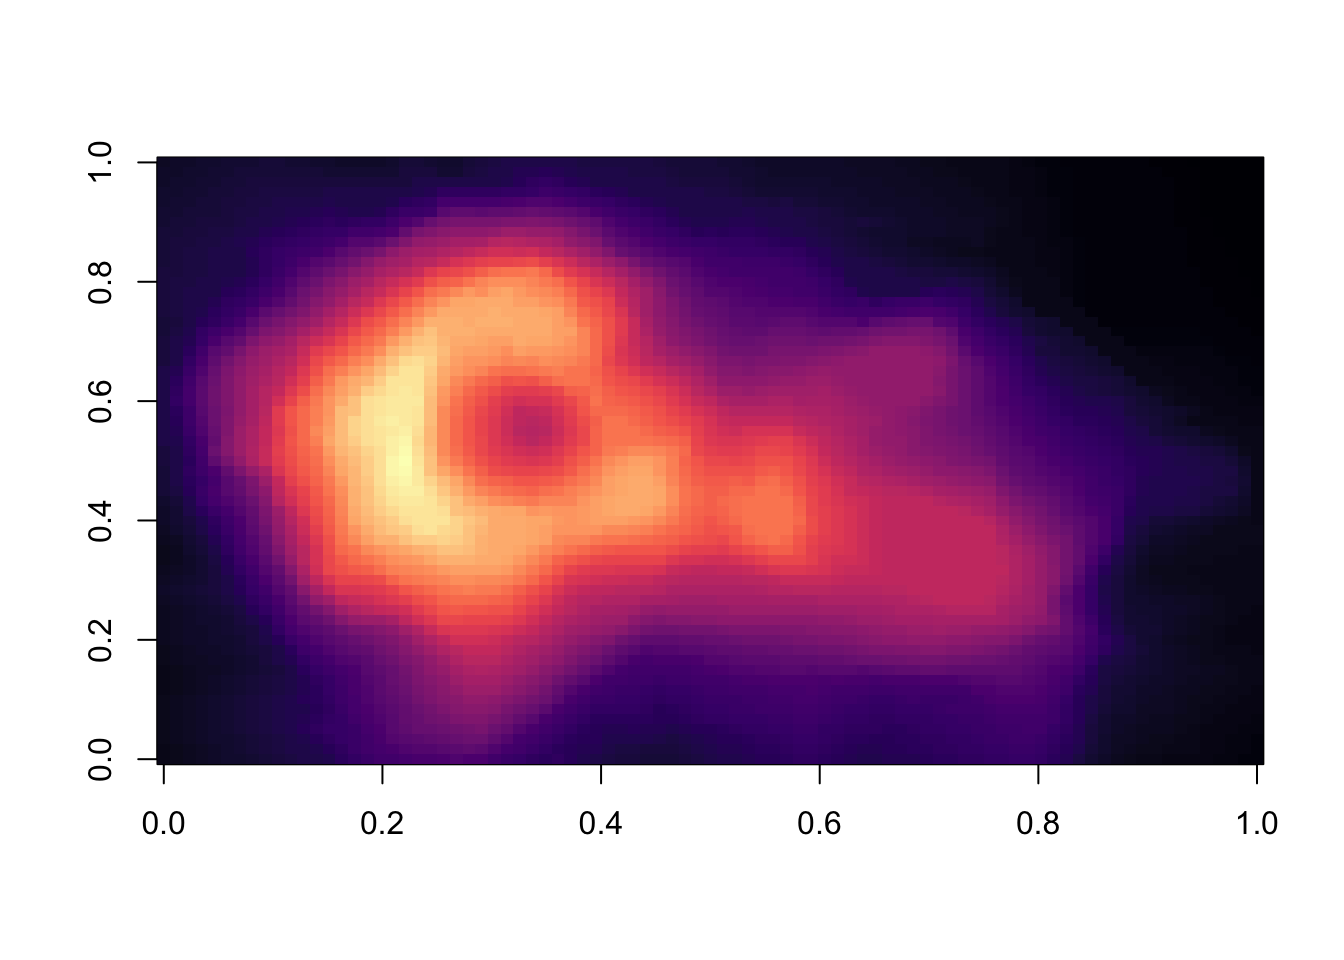
\includegraphics{figures/unnamed-chunk-8-1.png}
\caption{Figure}
\end{figure}

\hypertarget{gganimate-animations}{%
\subsubsection{\texorpdfstring{\texttt{gganimate}
animations}{gganimate animations}}\label{gganimate-animations}}

Pedersen and Robinson (2022)

\begin{Shaded}
\begin{Highlighting}[]
\FunctionTok{library}\NormalTok{(ggplot2)}
\FunctionTok{library}\NormalTok{(gganimate)}
\FunctionTok{library}\NormalTok{(gapminder)}

\FunctionTok{ggplot}\NormalTok{(gapminder, }\FunctionTok{aes}\NormalTok{(gdpPercap, lifeExp, }\AttributeTok{size =}\NormalTok{ pop, }\AttributeTok{colour =}\NormalTok{ country)) }\SpecialCharTok{+}
    \FunctionTok{geom\_point}\NormalTok{(}\AttributeTok{alpha =} \FloatTok{0.7}\NormalTok{, }\AttributeTok{show.legend =} \ConstantTok{FALSE}\NormalTok{) }\SpecialCharTok{+} \FunctionTok{scale\_colour\_manual}\NormalTok{(}\AttributeTok{values =}\NormalTok{ country\_colors) }\SpecialCharTok{+}
    \FunctionTok{scale\_size}\NormalTok{(}\AttributeTok{range =} \FunctionTok{c}\NormalTok{(}\DecValTok{2}\NormalTok{, }\DecValTok{12}\NormalTok{)) }\SpecialCharTok{+} \FunctionTok{scale\_x\_log10}\NormalTok{() }\SpecialCharTok{+} \FunctionTok{facet\_wrap}\NormalTok{(}\SpecialCharTok{\textasciitilde{}}\NormalTok{continent) }\SpecialCharTok{+}
    \CommentTok{\# Here comes the gganimate specific bits}
\FunctionTok{labs}\NormalTok{(}\AttributeTok{title =} \StringTok{"Year: \{frame\_time\}"}\NormalTok{, }\AttributeTok{x =} \StringTok{"GDP per capita"}\NormalTok{, }\AttributeTok{y =} \StringTok{"life expectancy"}\NormalTok{) }\SpecialCharTok{+}
    \FunctionTok{transition\_time}\NormalTok{(year) }\SpecialCharTok{+} \FunctionTok{ease\_aes}\NormalTok{(}\StringTok{"linear"}\NormalTok{)}
\end{Highlighting}
\end{Shaded}

\hypertarget{plotly-interactives}{%
\subsubsection{\texorpdfstring{\texttt{plotly}
interactives}{plotly interactives}}\label{plotly-interactives}}

Sievert (2020)

\begin{Shaded}
\begin{Highlighting}[]
\FunctionTok{library}\NormalTok{(rjson)}
\FunctionTok{library}\NormalTok{(plotly)}

\NormalTok{url }\OtherTok{\textless{}{-}} \StringTok{"https://raw.githubusercontent.com/plotly/datasets/master/geojson{-}counties{-}fips.json"}
\NormalTok{counties }\OtherTok{\textless{}{-}}\NormalTok{ rjson}\SpecialCharTok{::}\FunctionTok{fromJSON}\NormalTok{(}\AttributeTok{file =}\NormalTok{ url)}
\NormalTok{url2 }\OtherTok{\textless{}{-}} \StringTok{"https://raw.githubusercontent.com/plotly/datasets/master/fips{-}unemp{-}16.csv"}
\NormalTok{df }\OtherTok{\textless{}{-}} \FunctionTok{read.csv}\NormalTok{(url2, }\AttributeTok{colClasses =} \FunctionTok{c}\NormalTok{(}\AttributeTok{fips =} \StringTok{"character"}\NormalTok{))}
\NormalTok{fig }\OtherTok{\textless{}{-}} \FunctionTok{plot\_ly}\NormalTok{()}
\NormalTok{fig }\OtherTok{\textless{}{-}}\NormalTok{ fig }\SpecialCharTok{\%\textgreater{}\%}
    \FunctionTok{add\_trace}\NormalTok{(}\AttributeTok{type =} \StringTok{"choroplethmapbox"}\NormalTok{, }\AttributeTok{geojson =}\NormalTok{ counties,}
        \AttributeTok{locations =}\NormalTok{ df}\SpecialCharTok{$}\NormalTok{fips, }\AttributeTok{z =}\NormalTok{ df}\SpecialCharTok{$}\NormalTok{unemp, }\AttributeTok{colorscale =} \StringTok{"Viridis"}\NormalTok{,}
        \AttributeTok{zmin =} \DecValTok{0}\NormalTok{, }\AttributeTok{zmax =} \DecValTok{12}\NormalTok{, }\AttributeTok{marker =} \FunctionTok{list}\NormalTok{(}\AttributeTok{line =} \FunctionTok{list}\NormalTok{(}\AttributeTok{width =} \DecValTok{0}\NormalTok{),}
            \AttributeTok{opacity =} \FloatTok{0.5}\NormalTok{))}
\NormalTok{fig }\OtherTok{\textless{}{-}}\NormalTok{ fig }\SpecialCharTok{\%\textgreater{}\%}
    \FunctionTok{layout}\NormalTok{(}\AttributeTok{mapbox =} \FunctionTok{list}\NormalTok{(}\AttributeTok{style =} \StringTok{"carto{-}positron"}\NormalTok{, }\AttributeTok{zoom =} \DecValTok{2}\NormalTok{,}
        \AttributeTok{center =} \FunctionTok{list}\NormalTok{(}\AttributeTok{lon =} \SpecialCharTok{{-}}\FloatTok{95.71}\NormalTok{, }\AttributeTok{lat =} \FloatTok{37.09}\NormalTok{)))}
\NormalTok{fig}
\end{Highlighting}
\end{Shaded}

\hypertarget{inline-seaborn-figures}{%
\subsubsection{\texorpdfstring{inline \texttt{Seaborn}
figures}{inline Seaborn figures}}\label{inline-seaborn-figures}}

\emph{(with captions, re-scaled, id for ref)}

\hypertarget{code}{%
\subsection{code}\label{code}}

\hypertarget{python-codeblock-need-to-figure-out-how-to-output-figstats}{%
\subsubsection{\texorpdfstring{\texttt{Python}
codeblock}{Python codeblock}}\label{python-codeblock-need-to-figure-out-how-to-output-figstats}}

\emph{(demo numpy/pandas/scipy/sklearn/keras/tensorflow)}

\emph{(T: figure out how to output fig/stats)}

\begin{Shaded}
\begin{Highlighting}[]
\ImportTok{import}\NormalTok{ numpy }\ImportTok{as}\NormalTok{ np}

\CommentTok{\# data input}
\NormalTok{datapath }\OperatorTok{=} \StringTok{\textquotesingle{}/Users/matthewbain/Documents/Math/courses/semester II/PHYS 3G03/3G0{-}assignments/HW 3/code/\textquotesingle{}}
\NormalTok{csvname }\OperatorTok{=}\NormalTok{ datapath }\OperatorTok{+} \StringTok{\textquotesingle{}breast\_cancer\_data.csv\textquotesingle{}}
\NormalTok{data1 }\OperatorTok{=}\NormalTok{ np.loadtxt(csvname, delimiter }\OperatorTok{=} \StringTok{\textquotesingle{},\textquotesingle{}}\NormalTok{)}

\CommentTok{\# get input and output of dataset}
\NormalTok{x }\OperatorTok{=}\NormalTok{ data1[:}\OperatorTok{{-}}\DecValTok{1}\NormalTok{, :]}
\NormalTok{y }\OperatorTok{=}\NormalTok{ data1[}\OperatorTok{{-}}\DecValTok{1}\NormalTok{:, :]}

\BuiltInTok{print}\NormalTok{(}\StringTok{"hello"}\NormalTok{)}
\end{Highlighting}
\end{Shaded}

\hypertarget{embedding-stuff}{%
\subsection{embedding stuff}\label{embedding-stuff}}

\hypertarget{spotify-playlist}{%
\subsubsection{Spotify playlist}\label{spotify-playlist}}

\hypertarget{soundcloud-mix}{%
\subsubsection{SoundCloud mix}\label{soundcloud-mix}}

\textless iframe width=``100\%'' height=``300'' scrolling=``no''
frameborder=``no'' allow=``autoplay''
src=``\url{https://w.soundcloud.com/player/?url=https\%3A//api.soundcloud.com/playlists/872489715\&color=\%23ff5500\&auto_play=false\&hide_related=false\&show_comments=true\&show_user=true\&show_reposts=false\&show_teaser=true\&visual=true}''

Fujinai · Corridors

\hypertarget{basic-building-blocks-of-statements}{%
\subsection{example body text (`organization of
ideas')}\label{basic-building-blocks-of-statements}}

\hypertarget{basic-building-blocks-of-statements-1}{%
\subsubsection{Basic building blocks of
statements}\label{basic-building-blocks-of-statements-1}}

\emph{(i.e., linguistic/mathematical/etc. expressions of ideas)}

\begin{enumerate}
\def\labelenumi{\arabic{enumi})}
\item
  `first-order' statements

  \begin{itemize}
  \tightlist
  \item
    = basic true/false statements (e.g., y is/is not --- note: can think
    of a statement like this as expressing that an object possesses a
    property or `does something', which is roughly equivalent to an
    equivalence between object and property or object and operation),
    sometimes with categorical qualifiers (e.g., all, some, etc.)
  \item
    note: can think of these as definitions
  \item
    more complex definitions (e.g., of more complex objects/operations)
    may combine multiple of these using logical connectives (see
    {[}3{]})
  \item
    we can call these `compound statements' of first-order statements
  \end{itemize}
\end{enumerate}

\hypertarget{actionable}{%
\section{Actionable}\label{actionable}}

\begin{itemize}
\item[$\square$]
  item 1

  \begin{itemize}
  \tightlist
  \item[$\square$]
    item 1b
  \end{itemize}
\item[$\square$]
  item 2
\end{itemize}

\hypertarget{scraps}{%
\section*{Scraps}\label{scraps}}
\addcontentsline{toc}{section}{Scraps}

\hypertarget{refs}{}
\begin{CSLReferences}{1}{0}
\leavevmode\vadjust pre{\hypertarget{ref-azzalini1990look}{}}%
Azzalini, Adelchi, and Adrian W Bowman. 1990. {``A Look at Some Data on
the Old Faithful Geyser.''} \emph{Journal of the Royal Statistical
Society: Series C (Applied Statistics)} 39 (3): 357--65.

\leavevmode\vadjust pre{\hypertarget{ref-gganimate}{}}%
Pedersen, Thomas Lin, and David Robinson. 2022. \emph{Gganimate: A
Grammar of Animated Graphics}.

\leavevmode\vadjust pre{\hypertarget{ref-citeR}{}}%
R Core Team. 2020. \emph{R: A Language and Environment for Statistical
Computing}. Vienna, Austria: R Foundation for Statistical Computing.
\url{https://www.R-project.org/}.

\leavevmode\vadjust pre{\hypertarget{ref-sievert2020interactive}{}}%
Sievert, Carson. 2020. \emph{Interactive Web-Based Data Visualization
with r, Plotly, and Shiny}. CRC Press.

\end{CSLReferences}

\end{document}
